\subsubsection*{Software Testing 14.11}
%WARUM SOLLTE GETESTET WERDEN´?
%WIESO END2END UND UNIT TEST?
%PROJEKTE SCHREITERN WEGEN MANGELHAFTE TESTING \%
%Einer der Gründe dafür ist, dass das Risiko, gar nicht oder zu wenig zu testen, erkannt wurde.
%Unter anderem, weil es klar/verstanden wurde, wie riskant ist, Testaktivitäten zu überspringen oder nicht genug Testing durchzuführen.
In der Vergangenheit haben Unternehmen das Risiko bei der Entwicklung ihrer Projekte unterschätzt. Die waren gezwungen, ihren Betrieb zu unterbrechen, oder haben aufgrund von Fehlern in ihren Anwendungen Kunden verloren. Beispiele dazu sind Starbucks im Jahr 2015, der gezwungen war, etwa 60\% der Filialen in den USA und Kanada wegen eines Softwarefehlers in seinem Kassensystem zu schließen{\cite{QS1}} oder Nissan im Jahr 2014 als fast 1 Million Fahrzeuge wegen eines Softwarefehlers in den Airbag-Sensoriksystemen zurückgeziehen musste{\cite{QS2}}. Neben der Verringerung des Risikos der oben genannten Situationen bietet das Software-Testing weitere Vorteile. Zu diesen Vorteilen gehören eine Erhöhung der Softwarequalität, die Trennung der zwischen Software-Testing und -entwicklung, bessere Chancen, Fehler zu entdecken, bevor die Kunden sie entdecken und vieles mehr. Aus diesem Grund wurden Unit-Tests für das Backend und End2End für das Frontend vorgesehen. 
\\
\subsubsection*{Unittest}
Auch als Komponententest bekannt, wird diese geschrieben, um die richtige Funktionsweise einer Codeeinheit zu prüfen. In den meisten Programmiersprachen ist das eine Funktion, ein Unterprogramm oder eine Methode. Für dieses Projekt wurde das Jest Framework verwendet. 
Sowohl Cypress als auch Jest stehen an der Spitze der Liste, wenn es um Test-Frameworks geht{\cite{QS3}}.
%Before/after all; damit der Zustand zurücksetzen kann.
%Ein TF darf nur 1 Sache testen. 
%1 Beispiel erläutern (User)
%Screenshot von Ergebnisse
%Beschreibung von Screenshot: 1. Zeile gibt an

\subsubsection*{End-to-End Testfälle}
Cypress IO ist ein Testautomatisierungswerkzeug für End-to-End-Tests und UI-Tests. 
\\
\subsubsection*{Testautomatisierung}
Die Automatisierung von Testfällen maximiert die Effizienz, wenn Testfälle in den Kontinuierliche-Integration(Continuous integration) Workflows einbezieht werden. Neuer Code kann automatisch getestet werden, z. B. jedes Mal, wenn ein neues Pull-Request erstellt wird.

\begin{figure}[ht]
	\centering
    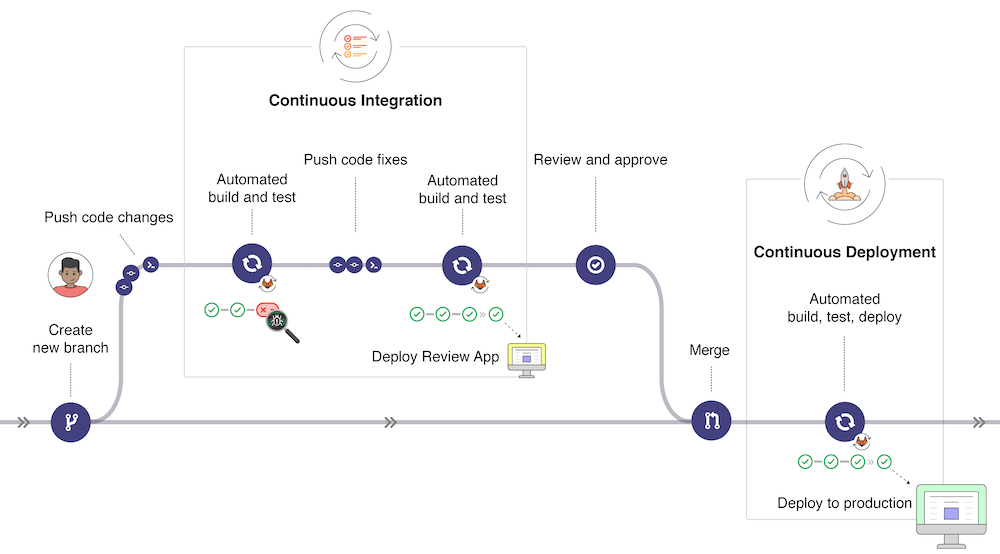
\includegraphics[width=\textwidth]{sources/Gitlab-CI.png}\cite{MG10}
	\caption{Gitlab-CI}
	\label{fig:Continuous_integration_workflow } {\cite{GLAB1}}
\end{figure}


\subsection*{Testing bei diesem Projekt}
\paragraph{}
Nachstehend einer Überblick über die Testfälle bei Cypress.
\\
Die \autoref{fig:Continuous_integration_workflow} zeigt den Ablauf, wenn ein neuer Branch erstellt wird und in diesen neuer Code eingebettet wird.
\begin{center}
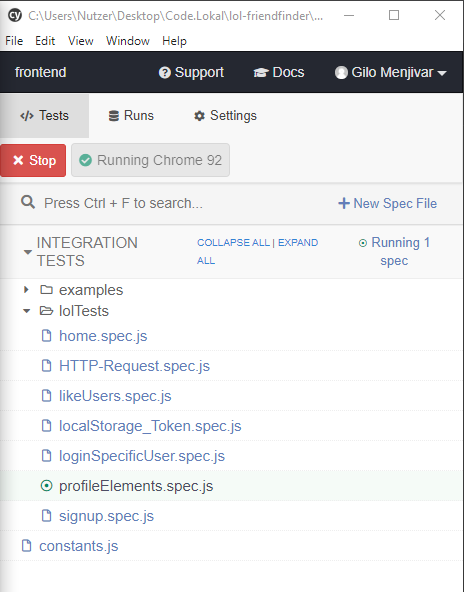
\includegraphics[scale=0.60]{Cy_Test_Cases}
\label{fig:Cy_Test_Cases}\\
\textbf{Abbildung \autoref{fig:Cy_Test_Cases}:} Testfälle in Cypress
\end{center}

\begin{center}
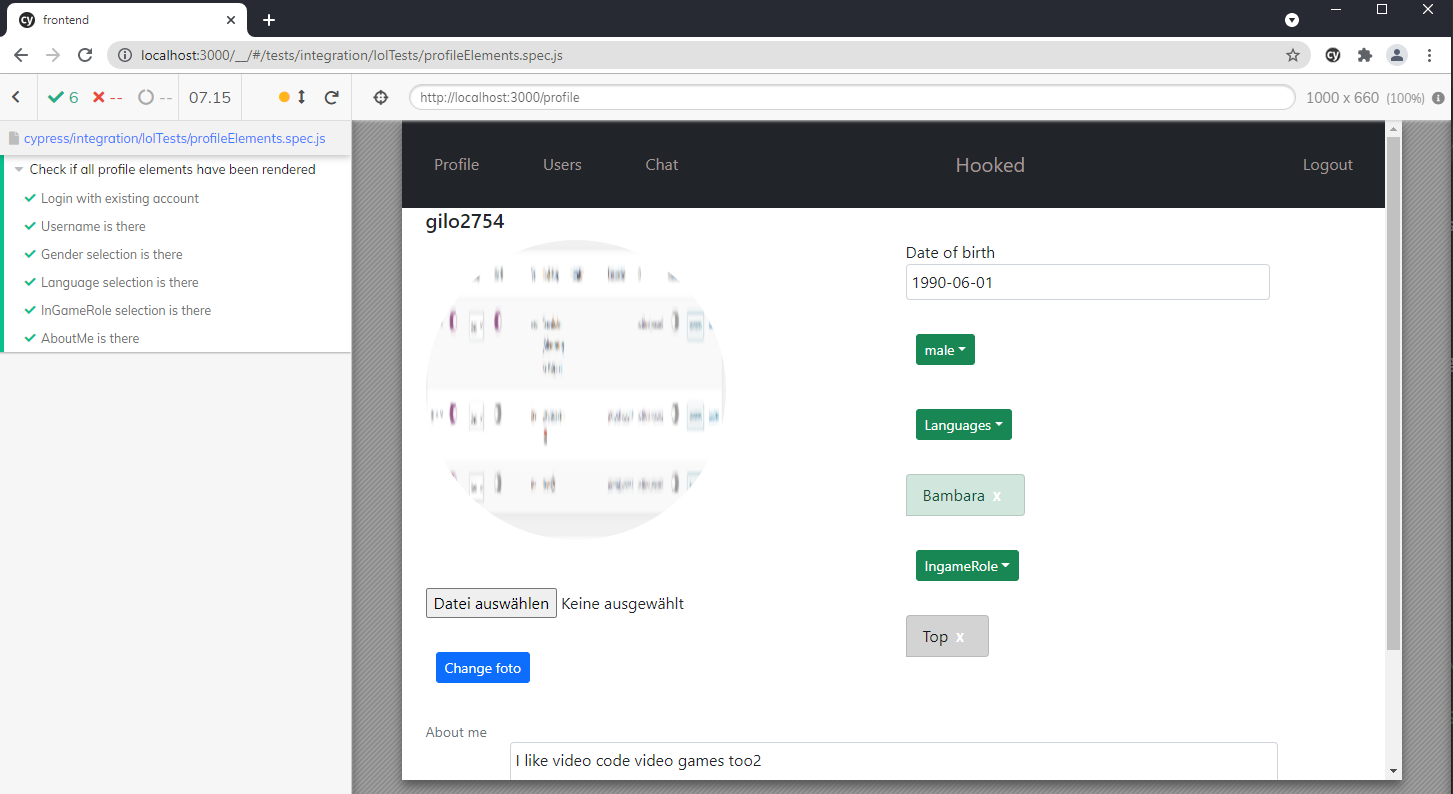
\includegraphics[scale=0.40]{Cy_Test_running}\label{fig:Cy_Test_running}
\textbf{Abbildung \autoref{fig:Cy_Test_running}:} Grafische Darstellung der verschiedenen Tests in Cypress
\end{center}


%Ergebnise der ganzen Testlauf

\subsection{Unit test (Backend)}
Für das Unit-Testing im Backend wird das Testingframework \textit{Jest} verwendet.
Dazu werden die Testkomponenten mit der Funktion \textit{describe} definiert.
Innerhalb einer Komponente werden die Testfälle selbst mit \textit{test} oder dem alias \textit{it} definiert.
Außerdem lassen sich Funktionen definieren, die nach oder vor jedem oder allen Testfällen ausgeführt werden sollen.
Dies ermöglicht atomare Tests, dessen Ergebnisse nicht durch andere Testfälle verfälscht werden und.
Die Testqualität wird somit erhöht.

Die Datenbankschemata werden mit Hilfe von \textit{mongodb-memory-server} getestet.
Dies erlaubt die Erstellung einer nicht-persistenten Datenbank im Speicher.
Die Datenbank ist initial leer und wird nach jedem Testfall gesäubert, um die Atomarität zu gewährleisten.
Durch Tests der Datenstruktur wird gewährleistet, dass es keine Abweichungen gibt zwischen den Daten, die erwartet werden und denen, die erhalten werden.
Tests der Middlewarefunktionen von Mongoose prüfen, ob komplexere Anwendungen, wie das Hashen des Passworts bei dessen Speicherung wie gewünscht ausgeführt werden.

Die Tests der GraphQl-Schnittstelle setzen voraus, dass die Datenbank wie gewünscht funktioniert und die gewünschten Daten liefert und speichert.
In verschiedenen Testfällen werden dazu die entsprechenden Resolver geprüft.
Dazu wird mit dem Paket \textit{apollo-server-integration-testing} ein Testclient erstellt, der mit \textit{query-} und \textit{mutation-}Abfragen ähnlich wie der richtige Klient abgefragt werden kann.
Der Testclient unterstützt keine Express-Middleware, welche im Projekt den Nutzer autorisiert und authentifiziert.
Diese Funktion musste daher nachgeahmt werden. 

\begin{comment}
Obwohl das Projekt relativ klein ist, wurde die Wichtigkeit von automatisierten Tests nicht unterschätzt.
\\
Für das Frontend wurden End-to-End Testfälle mit Cypress geschrieben.
Auf diese Weise ist es möglich in Sekundenschnelle festzustellen, ob etwas in unserer Anwendung defekt ist.

Ein Szenario, in dem dies hilfreich ist, ist, wenn eine Unterkomponente in anderen Komponenten verwendet wird.

Durch die Änderung der Unterkomponente kann sich diese in einer unerwünschten Weise verhalten.
\\
Das ist der Fall bei der Komponente AvatarImage.
Dies ist eine Funktionskomponente, die 3 Parameter erhält: Größe des Bildes, Bild-URL und Benutzername.

Zu Beginn des Projekts wurde nicht daran gedacht, die Größe des Bildes über einen Parameter dieser Funktion zu steuern. Im Laufe des Projekts wurde uns klar, dass wir die Logik in diesem Element wiederverwenden konnten.
\\
Innerhalb der Komponente wird geprüft, ob eine URL existiert, und wenn ja, wird das mit dem Link verbundene Bild gezeichnet. Falls es keine URL  angegeben wurde, werden die ersten beiden Buchstaben des Benutzernamens verwendet, um ein Standardsymbol zu erzeugen.

In der aktuellen Version des Codes wird diese Komponente in vier anderen Komponenten wieder verwendet.
Wenn das Projekt weiter wachsen würde, würde auch die Möglichkeit von Fehlern im Code zunehmen. Fehler zu finden, wäre in dem Fall aufwändiger.

Ohne automatisierte Tests, ist manuelles Testing nötig.
\\
Im Anhang 2 befindet sich ein Code-Auszug eines Testfälles End-to-End. 
\end{comment}
%%POSIBLEMENTE ESTE NO ES ELMEJOR EJ PUESTO QUE NO SE ESTA PROBANDO EL TAMANIO LAS IMAGENES EN LAS PRUEBAS DE CYPRESS
%% SIN EMBARGO EL HECHO DE REUTILIZAR LOGICA DE CIERTOS ELEMENTOS ES MUY RELEVANTE Y DEBERIA SER INCLUIDA EN OTRA PARTE %DEL REPORTE
%BUSCAR OTRO EJ. DONDE EL TESTING COBRA MAS RELEVANCIA

